\subsection{Problem statement}

We are given an empty set of of integers, and we want to be able to quickly add, remove, find operations.

\textbf{Approach 1}: The easiest (and slow) implementation could be to store all the elements in std::vector, then:

1. add = push\_back = $O(1)$.

2. find = $O(n)$.

3. remove = find + $O(1)$ (swap the found element with the last one and perform pop\_back).

\textbf{Approach 2 (with additional constraint)}: if all the elements are in the range of $[0, N)$, then we can allocate an array \textbf{is[N]}; then $is[x]$ indicates whether the element $x$ is present in the set or not, in this case all the required operations will work in $O(1)$.

\textbf{Idea solution}: the hash table is a data structure that allows to perform add, remove, and find in randomized $O(1)$.



\subsection{Hash table via std::list}

\begin{lstlisting}[language=C++]
std::list<int> table[N];

void add(int x) {
    table[x % N].push_back(x); // O(1)
}

auto /* = std::list<int>::iterator */ find(int x) {
    const auto& list = table[x % N];
    return std::find(list.begin(), list.end(), x); // works for O(list.size())
}

void remove(int x) {
    table[x % N].erase(find(x)); // works for find + O(1)
}
\end{lstlisting}

Instead of std::list you can use any container-like data structure, e.g., std::vector.

If there are $n$ elements present in the set and all of them are uniformly distributed, then each list will have on average $\frac{n}{N}$ elements $\implies$ if $n \leq N$ + elements are uniformly distributed, then all the operations will work in $O(1)$.

The uniform distribution of the elements is something we can potentially adjust via selecting a good hash function $f(x)$ for the elements (e.g., in the above we have used $f(x) = x \mod N$).



\subsection{Hash functions with probability of collision $O(\frac{1}{m})$}

\begin{statement}

    Functions $f(x) = x \mod N$ where $N$ is a prime number are good enough.

\end{statement}

In the following theorem we will show that there exist a special type of functions whose probability of collision is $O(\frac{1}{m})$ where $m$ is the capacity of the underlying hash table.

\begin{definition} \textbf{Universal family of hash functions}

    Given a universe of elements $U$.

    Let a hash function be defined as: $h: U \to \{0, 1, 2, ..., m-1\}$ for some $m$, or $h: U \to [m]$ ($[m] := {0, 1, 2, ..., m-1}$).

    $H = \{h: U \to [m]\}$ is called a \textbf{universal family} if:

    $\forall x, y \in U: \ x \neq y: \ |S| \leq \frac{|H|}{m}$ where $S := \{h \in H: h(x) = h(y)\}$. Perceive the $|S|$ as the number of hash functions that collide $x$ and $y$, then the inequation can be rewritten as:

    $\forall x, y \in U: \ x \neq y: \ \frac{|S|}{|H|} \leq \frac{1}{m}$ where $\frac{|S|}{|H|}$ is the probability of collision of $x$ and $y$ for the universal family $H$.

    "In other words, any two different keys of the universe collide with probability at most $\frac{1}{m}$ when the hash function $h$ is drawn uniformly at random from $H$." (\href{https://en.wikipedia.org/wiki/Universal_hashing}{wiki}).

\end{definition}

\begin{theorem}\textbf{Integer hashing}

    Let's consider a case where the values from the universe $U$ are finite (e.g., integer numbers in 64-bit computers), i.e. $U := \{0, 1, 2, ..., |U| - 1\}$.

    Select a prime $p$ which is $p \geq |U|$ and define:

    $h_{a, b}(x) := ((ax + b) \mod p) \mod m$ where $a, b$ are randomly chosen integers modulo $p$, and $a \neq 0$.

    The set $H := {h_{a, b}, \forall a \neq 0, b}$ is a \textbf{universal family}, i.e.:

    $\forall x, y \in U: x \neq y: \ Pr[\text{collision of $x$ and $y$ occurred}] \leq \frac{1}{m}$.

\end{theorem}

\begin{proof}

    Notice that the collision occurrs once $h_{a,b}(x) = h_{a,b}(y)$, $x \neq y$ which holds only when:

    $(ax + b) \% p \equiv_{m} (ay + b) \% p$

    $ax + b \equiv_{p} ay + b + im$ where $im \leq p-1$ because the right part of the equation is in $\{0, 1, 2, ..., p-1\}$, thus $i=1, 2, ..., \frac{p-1}{m}$.

    $a (x-y) \equiv_{p} im$ since $x \neq y$, $x, y \in U = \{0, 1, ..., |U|-1\}$ and $p \geq |U|$, and $p$ - prime, then $(x-y) \not\equiv_{p} 0$, thus the $(x-y)^{-1}$ exists:

    $a \equiv_{p} im \cdot (x-y)^{-1}$ - collision happens once the right and the left parts are equal. For every $i=1, 2, ..., \frac{p-1}{m}$ the equality takes place in exactly single value of $a$ because $a=1, 2, ..., p-1$, thus the probability of the collision is $Pr=\frac{\#i}{\#a} = \frac{\frac{p-1}{m}}{p-1} = \frac{1}{m}$.

    Thus, we have $Pr[\text{collision of $x$ and $y$ occurred}] \leq \frac{1}{m}$ $\implies$ $H$ is a universal family.

\end{proof}

\subsection{Open addressing collision resolution}

The implementation utilizes the cyclic array. A hash function is used to get the initial position in the array of the element $x$, next we move strictly right (modulo the capacity of the cyclic array) until we find a position in which either no element present or the element $x$ locates:


\begin{lstlisting}[language=C++]
int h[N]; // hash table

// h[i] = 0  : an empty cell
// h[i] = -1 : deleted element
// h[i] > 0  : there is an element

int getIndex(int x) { // get index by an element, require x > 0
    int i = x % N;
    while (h[i] && h[i] != x) {
        i = (i + 1) % N;
    }
    return i;
}

void add(int x) {
    h[getIndex(x)] = x;
}

void remove(int x) {
    // notice that the cell does not become empty!
    // marking a cell as empty will break the algorthm! see below
    h[getIndex(x)] = -1; // requires x != -1
}

int find(int x) {
    return h[getIndex(x)] != x;
}
\end{lstlisting}

\textbf{Why marking cells as removed is important}:

Suppose we mark a cell as empty once element is removed, then let's consider the following scenario:

You have $2$ elements $x$ and $y$ which are about to be added into the hash table $T$, and it turns out that the hash function $h$ over the elements results in $h(x) = h(y)$. Let's execute the following sequence of operations:

1. Suppose $T$ is empty.

2. $add(x)$ - adds $x$ at the position $i$.

3. $add(y)$ - adds $y$ at the position $i+1$ because $h(x) = h(y)$, thus the algorithm will traverse right until a free cell is found.

4. $remove(x)$ - marks the position $i$ as empty.

5. $find(y)$ - returns \textbf{false} because $h(y) = h(x) = i$, the cell $T[i]$ is marked to be empty, thus the find method says no $y$ found in the $T$.


\begin{center}
    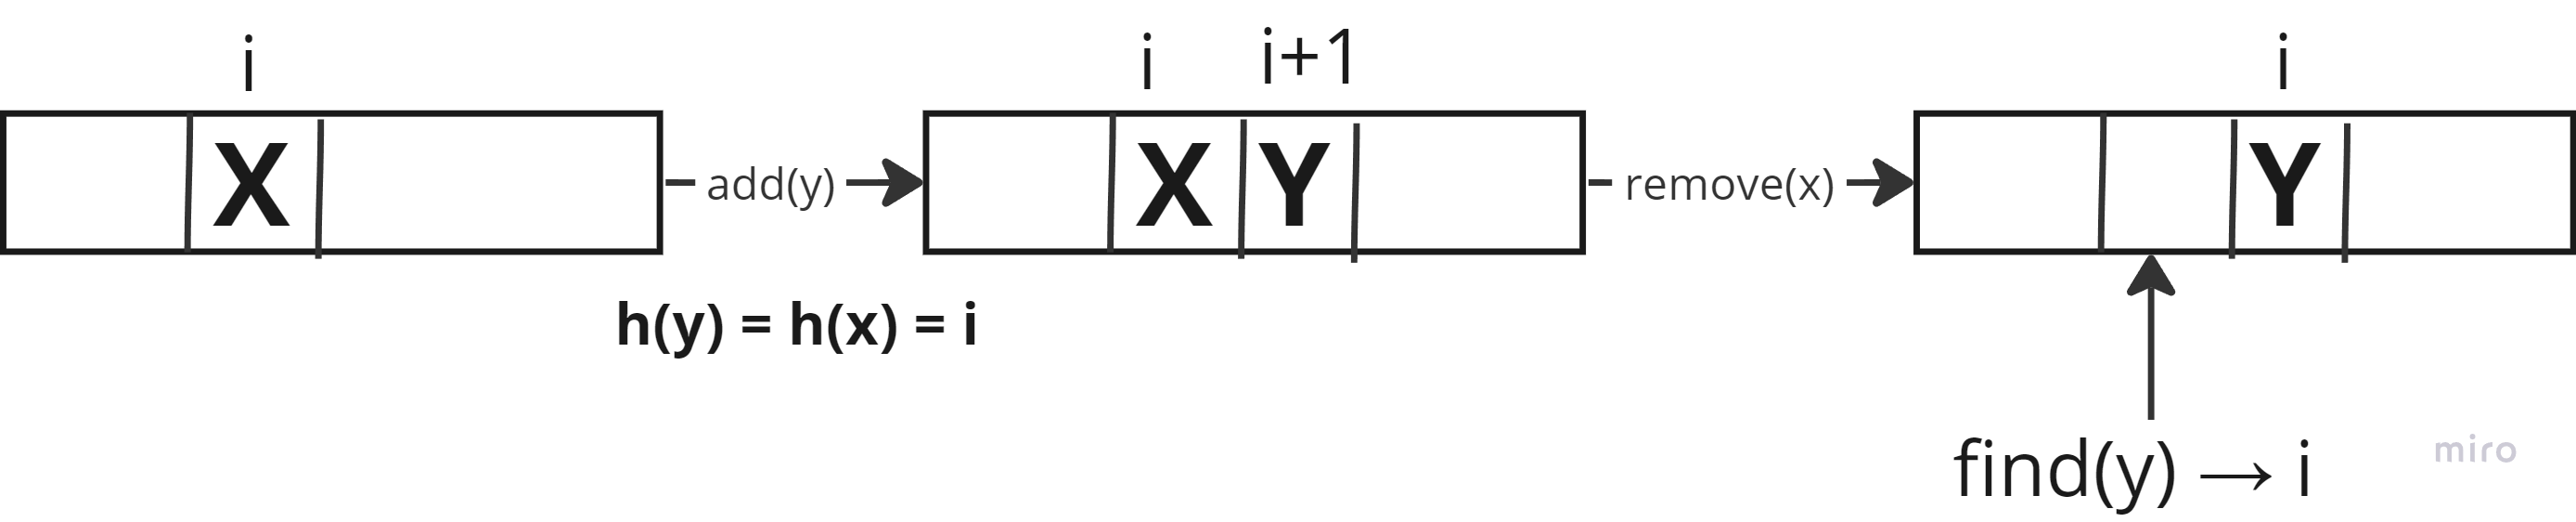
\includegraphics[scale=0.15]{./assets/11-hash-table/1.png}
\end{center}


\begin{lemma}
    If the hash table with open addressing of size $N$ has $\alpha N$ occupied cells ($\alpha < 1$), then the mathematical expectation $E$ of the time of \textbf{getIndex} $\leq \frac{1}{1-\alpha}$.

    For example, if there are only half of the elements occupied, i.e. $\alpha = \frac{1}{2}$, then on average each operation will require $\leq 2 = O(1)$ of time.
\end{lemma}

\begin{proof}

    Suppose that the free cells are distributed uniformly due to the hash function being good enough (no proof for it; oftentimes holds if you do not encounter an anti-test for your solution where all elements would have the same hash value).

    The worst case is when the element $x$ is not present in the table. In this case, on each iteration of the \textbf{while}-loop of \textbf{getIndex} the probability to \textbf{not stop} equals to $\frac{\alpha \cdot N}{N} = \alpha$ (due to the supposed uniform distribution).

    The probability to not stop even after $k$ iterations is $\alpha^k$, i.e. we will make $k$-th step with the probability of $\alpha^k$. Then, the execution time will be:

    $T = \text{mathematical expectation $E$ of the number of steps made} =$
    $= 1 + \sum_{k=1}^{+\infty} Pr[\text{the $k$-th step was made}] = 1 + \alpha + \alpha^2 + \alpha^3 + ... = \frac{1}{1-\alpha} $

\end{proof}

\subsubsection{Hash table overflow}

If $\alpha$ becomes too big the operations start to work slower:

1. $\alpha = 1$: no free cells, \textbf{getIndex} will infinitely serach for a free cell. How to resolve this problem?

Once $\alpha > \frac{2}{3}$ let's double the size of the underlying cyclic array and in linary time insert the elements into the new allocated buffer. During copying we will of course skip the cells marked as removed (i.e. $T[i] = -1$) $\implies$ the removed cells occupy the additional space only until the next sizing doubling takes place (i.e. there will be no removed cells bloating inside the hash table).

\subsection{Comparison of the approaches}

Overall, we have discussed two types of the hash table, let's compare them in terms of the required memory and time:

Suppose we store $x$ bytes for an object (element) and a pointer requires $8$ bytes, then our hash tables use for $n$ elements:

1. List-based approach (exactly $n$ lists): $8n (\text{pointers to $n$ lists}) + n \cdot (x + 8) (\text{every list has an element and a pointer to next}) = n \cdot (x+16)$ bytes.

2. Open addressing approach (having an additional capacity of $\frac{3}{2}$): $\frac{3}{2} \cdot n \cdot x$ bytes.

Time complexity:

1. List-based solution: requires to make on averange $2$ lookups, one for a list and one for an element inside the selected list.

2. Open addressing solution: requires on average $1$ lookup.


\subsection{STL implementation}

STL implementation uses list-based approach, thus if you write your own solution with open addressing it will work almost twice faster on average.

1. \textbf{std::unordered\_set<int> h} - hash table that stores the set of integers.

\textbf{Use}:

1. \textbf{std::unordered\_set<int> h(N)} - create a hash table with the capacity of $N$ cells.

2. \textbf{h.count(x)} - check whether $x$ present.

3. \textbf{h.insert(x)} - add an element $x$ (no-op if already present).

4. \textbf{h.erase(x)} - remove an element $x$ (no-op if already not present).


2. \textbf{std::unordered\_map<int, int> h} - hash table that stores \textbf{std::pair<int, int>}.

\textbf{Use}:

1. \textbf{std::unordered\_map<int, int> h(N)} - create a hash table with the capacity of $N$ cells.

2. \textbf{h[i] = x} - $i$-th cell can be used as an array index, stores an association $i \to x$.

3. \textbf{h.count(x)} - check whether a pair with the first component being equal $i$ present ($i$ is a key).

4. \textbf{h.erase(x)} - remove a pair  with the first component being equal $i$ if present ($i$ os a key).

You may use \textbf{std::unordered\_map} as an array with arbitrary indices, it is oftentimes called an \textbf{associative array} because for each key $i$ there is an association with a value $x$.

Depending on the set initial capacity of the \textbf{std::unordered\_map} there exists an anti-test which makes the structure to work in linear time for an operation, thus, if there is a change that a testing system might have an anti-tests for the initial capacity $N$, it may be helpful to set the initial capacity to be an random value:

\begin{lstlisting}[language=C++]
int64_t randomTime() {
    std::random_device rd;  // Obtain a random number from hardware
    std::mt19937 eng(rd()); // Seed the generator

    // Define the range of time (in seconds)
    std::uniform_int_distribution<> distr(0, 86400); // 86400 seconds in a day

    // Get the current time
    std::time_t currentTime = std::time(nullptr);

    // Generate a random offset from the current time
    std::time_t randomTime = currentTime + distr(eng);
    return static_cast<int64_t>(randomTime);
}

unordered_map<int, int> h(N + randomTime() % N);
\end{lstlisting}